%-------------------------------------------------------
% Gamification Techniques
%-------------------------------------------------------

Gamification consists of using game developing techniques in non-game environments, such as social networks, e-health, e-commerce, and educational systems \cite{kapp2012gamification,Deterding2011,Gamification_definition}. The techniques and resources used in digital games have elements
capable of (i) motivate users,(i) hold their interest, and (iii) challenge them
to solve problems. In gamification approaches, these elements are
not the center of the system, instead these elements have the purpose of attract users and motivate them to keeping using it \cite{Deterding2011}. Foursquare application (Figure~\ref{fig:foursquere}) is an
example of a gamified system. Foursquare is not a game. Foursquare is a location-based
social network, which reached 10 billion “check-ins” in 2016 \cite{Blankfeld2017forbes}.
Foursquare allows users to check-in at venues using a device specific
front-end to the application (e.g., mobile website), each
check-in might award the user with user-points or “badges”. To summarize, despite not being a game, Foursquare has a set of features usually found in games: points, badges, leaderboards, for instance, with the intent to captivate, motivate and keep users interested in the application, 

% Gamification
\begin{figure}[h!]
\caption{Foursquare screens, from left to right, list of user's check-ins and badges earned. }
\centering
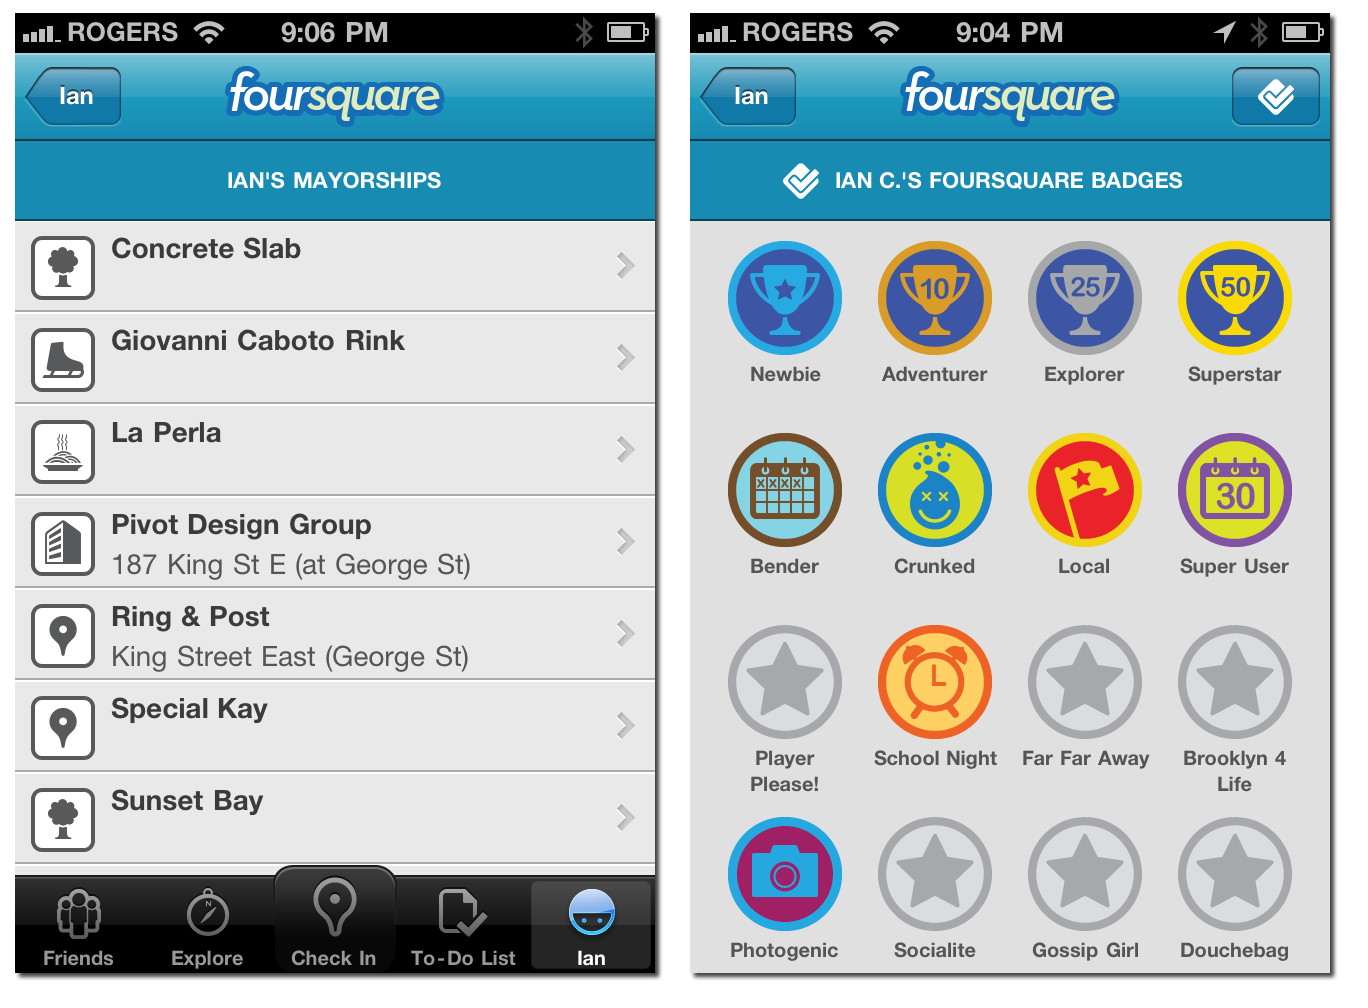
\includegraphics[width=0.4\textwidth]{foursquare}
\label{fig:foursquere}
\end{figure}

\textit{Explicar pointification, 
Argumentar que evoluiu agora trend personalização.}

For means of clarification, before presenting important topics related to this research, we first make some considerations about concepts usually related to the term "game". The following discussion is not comprehensive, and it is only intended to clarify and narrow down our definition of gamification. A more comprehensive and deep discussion can be found in \citeauthor{Deterding2011}.


It is worth to point out that the current thesis focus on covering research that explicitly match our definition of Gamification.
Therefore, we are not considering research based on playful design, serious games, video games, or other uses of game concepts in educational contexts.

%-------------------------------------------------------
% Game Design Elements
%-------------------------------------------------------
\section{Game Design Elements}
\label{sec:Game_Design_Elements}

\sigla{GDE}{Game design elements} is a term used to cover a broad list of game mechanics, dynamics, and aesthetics used in the design and development of games \cite{kapp2012gamification,Gamification_of_Collaborative_Learning}. In the gamification process, these elements work as motivational \textit{affordances} to deliver gameful experiences to the users, and as a consequence, trying to influence their behavior \cite{Does_Gamification_Work}. 
A high-level definition of GDE categories, usually found in the literature, is as it follows: 

\begin{itemize}
\item \textbf{Mechanics} They define the rules, actions and behaviors allowed in the game, and they are characterized by game components at the level of data representation and algorithms:
\subitem Examples: Rules, goals (objectives), levels, number of players. 
\item \textbf{Dynamics} characterize the run-time behavior of the mechanics reacting on player inputs;
\subitem Examples: Feedback, conflict, competition, cooperation, time pressure.
\item \textbf{Aesthetics} characterize the interaction with the game system (i.e., input-output and vice versa).
\subitem Examples: Sensation, fantasy, narrative, challenge, fellowship, discovery, expression.
\end{itemize}

According to \citeauthor{hunicke2004}, starting from the designer’s perspective,
the mechanics rise the dynamic system behavior, which in turn produces aesthetic experiences that will be consumed by the player.
However, from the player’s perspective, aesthetics set the \textit{tone} of the experience as a direct result of player's reaction to the dynamics, in turn, dynamics are paced by the available mechanics. For this reason it is important to have both perspectives in focus, and neglecting none of them.

% Video games or Digital games
\begin{figure}[h!]
\caption{Designers and players have different, but linked, perspectives of the game. Adapted from \cite{hunicke2004}}
\centering
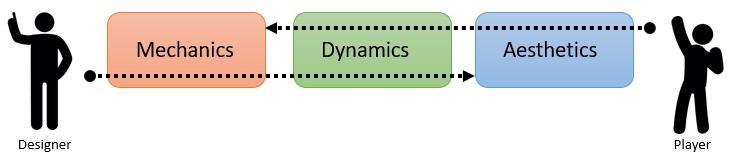
\includegraphics[width=0.8\textwidth]{mda_views}
\label{fig:mda_views}
\end{figure}

To illustrate how game elements can be linked, we will provide an example of scenario using the game element \textbf{Challenge}. Challenge is an example of aesthetic element, and it is a powerful one since it poises an obstacle between the player and the reward/victory. 
For instance, challenge can be created by the dynamic \textbf{time pressure}, where the player has limited time to accomplish a task. 
In turn, time pressure to exist depends of mechanics such as \textbf{rules specification} (e.g., how much time does the player have?) and \textbf{rules implementation} (e.g., algorithms and data). 
As an usage example of such approach, we can cite the Super Mario Bros \textsuperscript{\textregistered} game franchise. In many games of the franchise, the character Mario needs to reach the end of the stage before running out of time otherwise, the player will fail the challenge (Figure \ref{fig:mda}). Figure \ref{fig:duolingo} shows an example of the same usage, challenge based on time pressure, however in a non-game application. The application in question is Duolingo, a well known free language-learning platform. Duolingo is a successful example of how gamification can be skillfully applied to a system \cite{Huynh2016}. In the example, the learner needs to complete a task in an specific amount of time to be rewarded. 
% https://www.quora.com/How-effective-is-Duolingo-in-learning-a-language
% Figura Mario
\begin{figure}[h!]
\caption{Usage example of "challenge based on time pressure" in a game.}
\centering
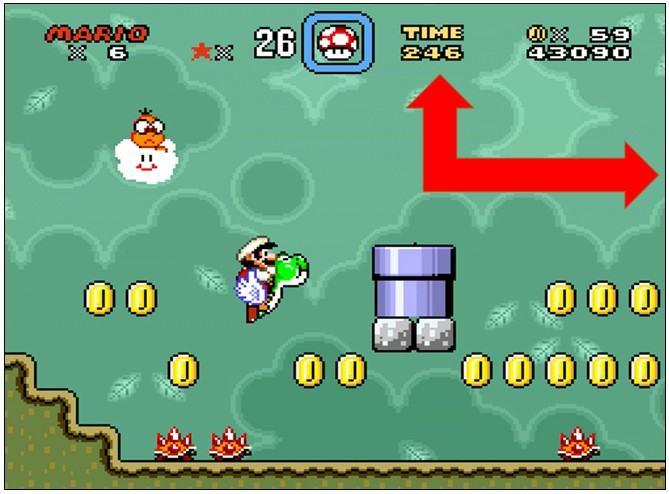
\includegraphics[width=0.4\textwidth]{mda}
\label{fig:mda}
\end{figure}

% Figura Duolingo
\begin{figure}[h!]
\caption{Usage example of "challenge based on time pressure" in a gamified application.}
\centering
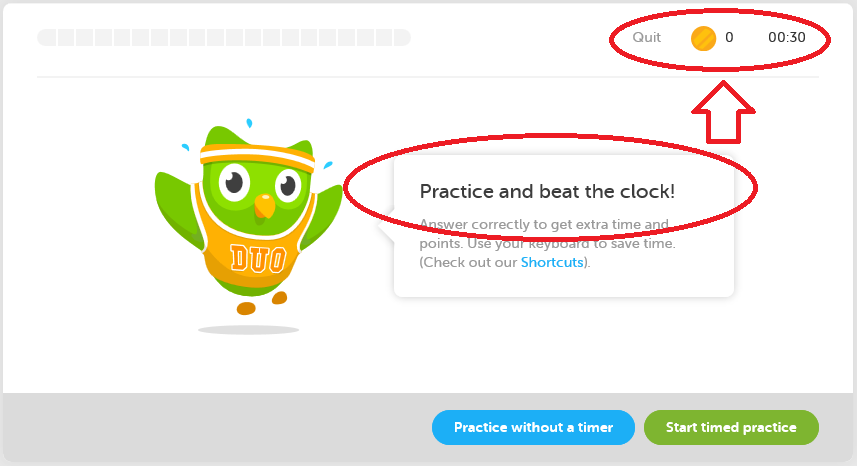
\includegraphics[width=0.6\textwidth]{duolingo2}
\label{fig:duolingo}
\end{figure}

GDE have been exhaustedly discussed in the gamification literature \cite{kapp2012gamification,robinson2013preliminary,werbach2012win,zichermann2010game,zichermann2011gamification,Ferro2013}.
Many researchers have tried to summarize these elements and create a unified taxonomy. However, up to this point, there is no consensus about an universal compilation. 
For this reason, 
there are several lists, conceptual frameworks, and guidelines with compilations of game design elements in the literature \cite{Ferro2013,A_Link_Between_Worlds}. 
Regardless the overlaps or parallels found in these lists, 
they can great differ from one to another making the design and implementation of gamification techniques harder \cite{Sailer2017}.

In this thesis, it is not our intention to propose a new compilation of game elements. So, we will stick with the game design elements shown in Table X . Although it is not an extensive compilation, all these elements have been extensively used in the game industry (i.e., best practices) \cite{ferro2016gamification}, and have been empirically evaluated in many gamification studies\cite{Sailer2017}. In addition, we will not try to explain the overlaps and relationships between each and all elements shown in Table 1. Instead, we are more interested in investigate how the selected game design elements can be harnessed to support constraint-based group formation.

Table 

%-------------------------------------------------------
% Player Types
%-------------------------------------------------------
\section{Player Typologies}
\label{sec:Player_Typologies}

The concept of player types is based on the assumption that different persons have different reactions given a certain game element \cite{fullerton2008}.
One of the first player typologies used in gamification was Bartle's Player Types \footnote{Richard Bartle created the model, the so called "Bartle's Player Test" was later implemented by Erwin Andreasen and Brandon Downey \cite{Bartle2009}}. However, since the publication of Bartle's seminal study, several other models have been proposed. In this section an overview of some important typologies in the context of this thesis is provided. 

\subsection{Bartle's Players Types}
\label{sec:Bartle_Players_Types}

Richard Bartle co-created a text-based game called \sigla{MUD}{Multi-User Dungeon}, the ancestor of today's \sigla{MMORPGs}{Massively Multiplayer Online Role-Playing Games}. 
He performed some observations in the game environment trying to figure out what players were looking for in the game (i.e., MUD). 
By analyzing the answers of a questionnaire and from observing players behaviors within the game, he conceived four player psychological portraits in a MUD: Killers, Achievers, Explorers and Socializers \cite{Bartle1996}. 
The taxonomy provided by \citeauthor{Bartle1996} are the foundations of player types research, but it has its limitations. 
For instance, Bartle's model was constructed using comparisons between scenarios that respondents must choose. 
As pointed by \citeauthor{yee2006motivations}, if a questionnaire has questions that force the respondent to choose between two scenarios, the answer may represent a dichotomy, and bias may occur towards various outcomes.
In addition, as explained by \citeauthor{Bartle2009}, the model was created to fulfill a different purpose and it was never intended to be used in the gamification domain.
For instance, \citeauthor{youtube_bartle} alert that the model might be incomplete for other domains than MUD's and as a consequence, designers might be "forced" to fit players in some available category  (i.e., therefore ignoring their personal traits) or even ignore "non-recognized" players types (i.e., players that do not "fit" any available types) \cite{Bartle2009}.


\subsection{BrainHex}
\label{sec:BrainHex}

According to \cite{bateman2011player}, the creation of robust and efficient player models need be rooted on trait theory of players preferences. 
Nevertheless, while research on psychometric typology for personality has a long history, player typology and trait theories of play are still in their infancy. 
BrainHex is a player satisfaction model build on previous efforts from the \sigla{DGD1}{Demographic Game Design model 1} and the \sigla{DGD2}{Demographic Game Design model 2} \cite{Nacke2014}. 
BrainHex build up on insights from neurobiological findings from these models and presents seven different archetypes of players: Seeker, Survivor, Daredevil, Mastermind, Conqueror, Socialiser, and Achiever. These archetypes are related to typologies such as Myers-Briggs \cite{myers1985manual}, and each one characterizes a specific player type.
The model was validated using data collected from a survey and comparing the demographic data to different BrainHex archetypes. Using the results of the psychometric orientation of respondents, they established a relationships between personality types and BrainHex archetypes. Data was collected from 50,000 respondents.

\subsection{Motivations for Playing Online}
\label{sec:motivations_for_playing_online}

Bartle's work was conducted in a exploratory fashion, however without the support of more robust statistical analysis \cite{yee2006motivations}. In the research conducted by \citeauthor{yee2006motivations}, a compilation of suitable motivations for playing in MMORPGs was created based on the literature (i.e., Bartle’s Player Types) and open-ended responses from several surveys. Using these information, a unified Likert-type survey was created. The surveys target audience was MMORPGs players. Data from 3200 respondents was collected and \sigla{FA}{factor analysis} was used to investigate the survey answers. At the beginning, 10 factors were extracted, and after performing another analysis of these 10 factors, three main factors were identified: Achievement, Social and Immersion. A summary of these results is shown in Table~\ref{tab:motivations_for_play_yee}.

% Please add the following required packages to your document preamble:
% \usepackage{booktabs}
\begin{table}[]
\centering
\caption{Main components of motivations to play in MMORPGs \cite{yee2006motivations}}
\label{tab:motivations_for_play_yee}
\begin{tabular}{@{}llc@{}}
\toprule
\textbf{Main Component} & \textbf{Subcomponent} & \multicolumn{1}{l}{\textbf{Factor Loading}} \\ \midrule
\textbf{Achievement} & Advancement & 0.85 \\
 & Mechanics & 0.77 \\
 & Competition & 0.68 \\
\textbf{Social} & Socializing & 0.74 \\
 & Relantionship & 0.62 \\
 & Teamwork & 0.76 \\
\textbf{Immersion} & Discovery & 0.72 \\
 & Role-Play & 0.70 \\
 & Customization & 0.66 \\
 & Escapism & 0.53 \\ \bottomrule
\end{tabular}
\end{table}

Motivations to Play \cite{yee2006motivations} has its roots on Bartle's model, but it differs from the original one in many points. 
The main difference between Yee's and Bartle's models is that instead of four main player types, \citeauthor{yee2006motivations} identified three main motivational components.
In addition, this three components are composed of subcomponents.
At the end, the model proposed by \citeauthor{yee2006motivations} does not attempt to identify in which archetype one player fits but rather to understand a set of components and how much each component can influence the player. 
By identifying the reasons that may arouse motivation to play, and by analyzing the results of the scoring system developed, one can also identify what can be deemed less attractive for such an individual. 

%-------------------------------------------------------
% Gamification Applied to Education
%-------------------------------------------------------
\section{Gamification Applied to Education}

Students motivation can play a vital role in students academic performance and achievements since it can influence the amount of effort and time spent in learning activities \cite{linehan2011}. So, there is a growing interest in gamification as well as its applications and implications in the field of education. This growing interest is mainly due to the potential of gamification techniques to motivate students during the process of learning \cite{Borges2014SAC}. 
However, gamification has been used in education with mixed results \cite{Berkling2013,Does_Gamification_Work,Mekler2015,Lieberoth2015,Dichev2017}. Some empirical findings indicate that gamification can increase motivation and engagement in students; other findings highlight that gamification can be a distraction to students; and therefore it may end up hindering learning. 

We carried out a systematic mapping study of research into gamification applied to education trying to identify studies covering and classifying the types of research being published and the most investigated topics in the area \cite{Borges2014SAC}. At first, we ran some searches using a combination of candidate keywords. These trial searches combined the keyword \textbf{gamification} with some synonyms related to \textbf{education} and \textbf{learning}. No limit of publication date was used (i.e., data range). Even though, due to the  small number of papers returned from the resulting strings, we decided that only the keyword \textbf{gamification} should be used. Later, by applying predefined inclusion  criteria, we manually selected only research in the education field. 
These decisions allowed us to analyze a greater number of papers, lowering the odds of leaving relevant studies out of our final set. Using gamification as keyword, we performed searches on electronic databases that are known to cover relevant scientific journals and articles from a wide variety of domains such as Computer Science, Education and Educational Research, Science, Engineering, Medicine and Psychology. Initially, we retrieved 357 primary papers. However, only 48 candidate papers were obtained after applying the inclusion and exclusion criteria based upon title and abstract. Finally, after going over introductions and conclusions, we ended up with a final set of 26 primary papers as shown in Table~\ref{tab:visao_geral_busca}. 

\begin{table}
[ht] \caption {Papers retrieved from each electronic
database, total of candidate studies, and the final
set.
. } \label{tab:visao_geral_busca} 
	\begin{center}
		\begin{tabular}
			{ | l | c | } 
				\hline\hline \textbf {Eletronic Database}  & \textbf{Number} \\
                \hline {ACM Digital Library} & 144 \\
				\hline {IEEE Xxplore} & 31 \\
				\hline {Elsevier (via Science Direct)} & 32  \\
				\hline {Springer} & 55 \\
                \hline {SCOPUS} & 95 \\
			\hline \hline \textsc{\textbf{Total}} & 357 \\
			\hline \textbf{Candidates} & 48 \\
			\hline \textbf{Final set} & 26 \\
			\hline\hline 
		\end{tabular}
	\end{center}
\end{table}

In this section we will summarize the main results of the literature review. Appendix~\ref{chapter:gf_mapping} contains supplementary information, such as: the rationale that backs up the literature review, statistics performed, and inforation about the final set of selected papers.






%-------------------------------------------------------
% Gamification in CSCL
%-------------------------------------------------------
\subsection{Gamification in CSCL}

To deal with this problem, it is necessary to design gamification to fit properly in individual and collaborative learning contexts. Unfortunately, there is a lack of studies on frameworks mapping game elements and learning theories to support the adequate design and application of gamification in education. 


There is a large amount of research on motivation and learning coming from different background; all demonstrating that motivation plays a vital role for individual learning. However, in the case of CSCL, learning is a more complex process, and despite this, research in this field has not been completely explored yet \cite{Motivation_in_a_computer-supported_collaborative_learning}. In [16] for instance, a meta-analysis of 41 studies investigated the effects of having choice (related to autonomy) and possible intrinsic motivation outcomes. These studies investigated both children and adults samples in different environments. The meta-analysis shows evidence that backs up the idea that enabling learners to choose from different learning alternatives enhanced not only intrinsic motivation, but also: task performance, effort, and perceived competence. However, in [9], they raised some concerns regards trying to manipulate students’ motivation. In this study, an experiment was performed and students' competence was evaluated (if appropriate) after completing specific collaborative tasks. The exploratory analyses presented evidences that the appraisal of one partner’s may have played an unexpected role increasing a free-riding behavior on students that did not received an appraisal. The authors assumed that the free-riding effect indicates that part of the participants lost their motivation, thus suggesting the influence of motivation also during CSCL. 


\subsection{Concluding Remarks}

Using this systematic method it is possible to aggregate and categorize primary studies, creating an overview of the research area in question \cite{petersen2008}. More recently, (i.e., February, 2017), we run a new search using the keyword "gamification". The purpose was to observe if the number of publications in the field has increased since the first search.  
Figure~\ref{fig:retrieved2017} shows the results of this search. As one can see, indeed there is a significant increase in the number of publications since 2013. 

% Figura retrieved in 2013 and 2017
\begin{figure}[h!]
\caption{Number of papers retrieved using the keyword "gamification".}
\centering
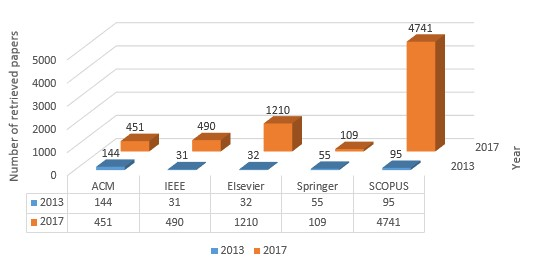
\includegraphics[width=0.8\textwidth]{retrieved2017}
\label{fig:retrieved2017}
\end{figure}

It is important to say we did not analyzed the additional publications returned in this last search in 2013. The numerical results were included here by way of comparison with the number of results observed in the previous search. Given the high number of returned papers, using a generic search string (i.e., gamification) as we did in 2013 may not be the optimal solution anymore. It will be necessary to review the research protocol (e.g., keywords, search string) to include new keywords that will help tuning the results towards research focused in education.
